\section{Aggregazione di unità allungate e polimeri}
\subsection{Unità monomeriche}\subsubsection{Aggregazione per legami ad idrogeno}\begin{frame}\frametitle{Unità monomeriche}\framesubtitle{Aggregazione per legami ad idrogeno}
\begin{columns}
\column{0.25\linewidth}  \vspace{-5pt}  \begin{figure}{\centering{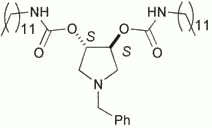
\includegraphics[width=1\textwidth]{sec3/carbammato.png}}}\end{figure}\vspace{-10pt}\begin{figure}{\centering{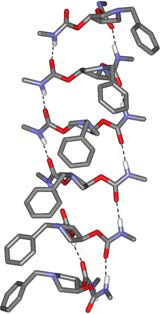
\includegraphics[width=0.8\textwidth]{sec3/carbammato-conformazione.png}}}\end{figure}
\column{0.75\linewidth} 
Il \textbf{monomero} in figura (con il cromoforo fenilico lontano dal centro chirale $\Rightarrow$ \textbf{non ha CD}) da aggregazione in strutture elicoidali.

I cromofori possono presentare \textbf{accoppiamento eccitonico} e dunque un CD indicativo dell'orientazione relativa. 

Gli aggregati danno fibre con avvolgimento osservabile tramite microscopia.

Si osserva \textbf{linearità} in esp. regola di maggioranza, avviene una \textbf{discriminazione enantiomerica} ossia una segregazione in \textbf{2 fibre} enantiomericamente \textbf{pure}. \cite{4}
\end{columns}
  \end{frame} 

\subsubsection{Aggregazione per interazione idrofobica}\begin{frame}\frametitle{Unità monomeriche}\framesubtitle{Aggregazione per interazione idrofobica}
\vspace{-5pt}\begin{columns}
\column{0.6\linewidth}\begin{figure}{\centering{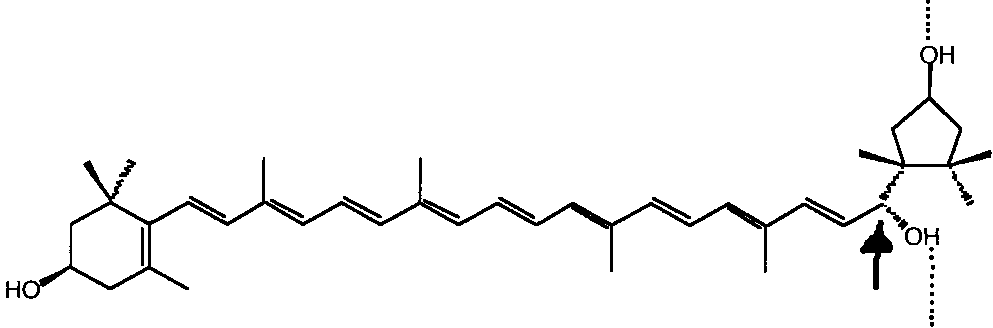
\includegraphics[width=0.8\textwidth]{sec3/carotenoide.png}}}\end{figure}\column{0.4\linewidth}\begin{figure}{\centering{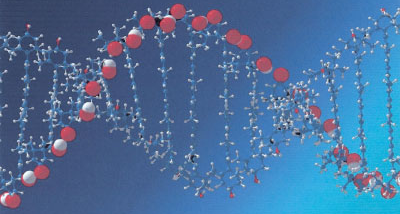
\includegraphics[width=0.9\textwidth]{sec3/carotenoide3d.png}}}\end{figure}\end{columns}
\vspace{10pt}
L'aggregazione avviene per \textbf{interazione idrofobica}, anche qui al CD si osserva l'accoppiamento eccitonico. 

A seconda della configurazione del carbonio indicato si possono avere \textbf{aggregati supramolecolari di tipo J o di tipo H} (J~=~aggregazione debole (testa-coda) e red shift dell'assorbimento; H~=~aggregazione compatta e blue shift). 

In figura l'aggregazione di tipo H in cui si ha una catena di legami ad idrogeno (evidenziati nelle figure). \cite{9}
  \end{frame} 

\subsection{Unità oligomeriche}\begin{frame}\frametitle{Unità oligomeriche}
           \begin{columns}
\column{0.5\linewidth}\begin{figure}{\centering{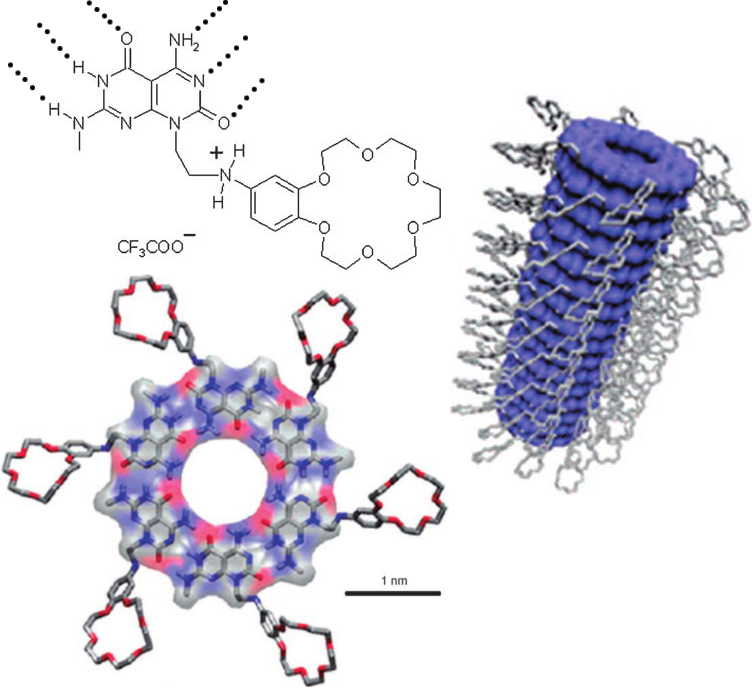
\includegraphics[width=1\textwidth]{sec3/oligomeri.png}}}\end{figure}\column{0.5\linewidth}   Il monomero \textbf{achirale} si assembla in dischi grazie ai legami ad idrogeno, dunque si aggrega in nanotubi. 

La \textbf{chiralità} viene \textbf{indotta} in modo non-lineare (cooperativa) aggiungendo un \textbf{amminoacido} chirale. \cite{8}
       \end{columns}      \end{frame}  

      \subsection{Unità polimeriche}\begin{frame}\frametitle{Unità polimeriche}
              \begin{columns}
\column{0.3\linewidth}\begin{figure}{\centering{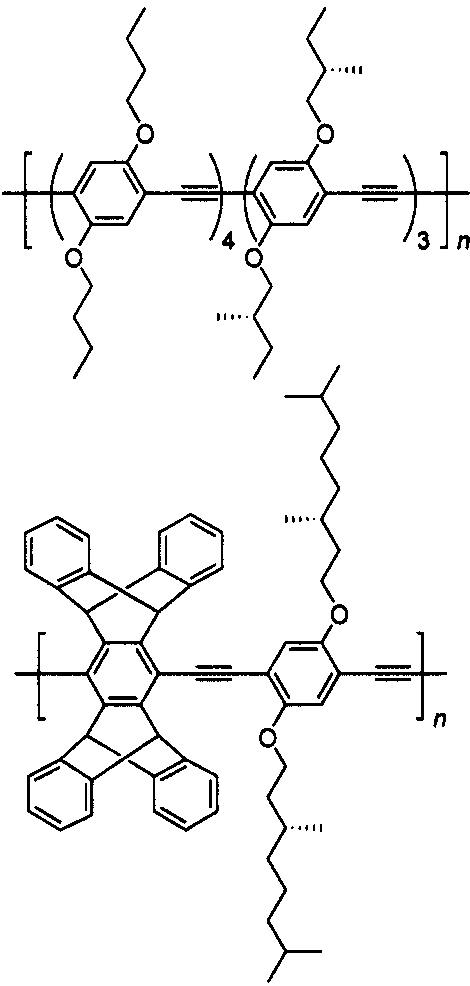
\includegraphics[width=0.9\textwidth]{sec3/polimeri.png}}}\end{figure}\column{0.7\linewidth} Utilizzare polimeri con della chiralità permette di \textbf{studiarne la conformazione utilizzando il CD} e di \textbf{impedire la formazione di aggregati allineati} allo scopo di ottenere proprietà optoelettroniche diverse (evitare il quenching di fluorescenza mantenendo l'accoppiamento elettronico intercatena). \cite{1} \end{columns}    
             \end{frame}    
